\documentclass{article}[11pt]
\usepackage[utf8]{inputenc}
\usepackage[T1]{fontenc}
\usepackage{float}
\usepackage[caption = false]{subfig}
\usepackage[final]{graphicx}
\usepackage{indentfirst}
\usepackage{fancyhdr}
\usepackage[a4paper,left=2cm,right=2cm,top=2.5cm,bottom=2cm]{geometry}
\usepackage{amsmath}
\usepackage{amssymb}
\usepackage{array}
\usepackage{pifont}
\usepackage{makecell}
\usepackage{xcolor}
\newcommand{\tabitem}{~~\llap{\ding{213}}~~}
\definecolor{pythonColor}{HTML}{B634F6}
\newcommand{\python}[1]{\textcolor{pythonColor}{\textit{#1}}}
\renewcommand{\headrulewidth}{0.5pt}
\renewcommand{\footrulewidth}{0.5pt}

% Propriétés de la matrice A:
%     Test à faire : ({Real, complex},
%                     {Pleine, Creuses{Bandes, Pas bandes}},
%                     {Symétrique} )


% Paramètres infuençant le conditionnement
%     SICN  : signed inverse condition number
%     SIGE  : signed inverse gradient error
%     Gamma : vol/sum_face/max_edge

\title{Éléments finis et conditionnement.}
\author{Romain Graux}
\date{Lundi, 28 Octobre 2019}

\begin{document}
\raggedbottom
\lhead{Romain Graux}
\rhead{Octobre 2019}
\lfoot{28681700}
\rfoot{Éléments finis et conditionnement}
\pagestyle{fancy}
\begin{center}
    \huge{{\textbf{Analyse Numérique : Devoir 1}}}
    
    \Huge{\textit{\textbf{Éléments finis et conditionnement}}}
\end{center}
\vspace{0.7cm}

\section{Propriétés de la matrice \textit{A}}

Ces données ont été obtenues par le biais de la fonction \python{all\_test}\textit{()} contenue dans le fichier \textit{mysolve.py}. Tous les tests ont été faits sur un raffinement tel que \python{ref}$ = 2$, ce qui correspond à \textit{2000} éléments et un \python{$\mu_r$} de $100$.

\begin{center}
\begin{tabular}{|p{1cm}|p{4cm}|p{4cm}|}
    \hline
    & \makecell{\textit{freq$=$0}}      & \makecell{\textit{freq$\neq $0}} \\
    \hline
    \makecell{\textit{vel$=$0}}
    & \makecell{\textbf{Statique}}      & \makecell{\textbf{Harmonique}} \\
    &                                   &                                \\
    & Réelle                            & Complexe                       \\
    & Symétrique                        & Symétrique                     \\
    & Définie positive                  & Définie positive               \\
    & Creuse                            & Creuse                         \\
    & Pas à bandes                      & Pas à bandes                   \\
    & Hermitienne                       & Non hermitienne                \\
    & Inversible                        & Inversible                     \\
    & Non unitaire                      & Non unitaire                   \\
    &                                   &                                \\
    \hline
    \makecell{\textit{vel$\neq $0}}
    & \makecell{\textbf{Stationnaire}}  & \makecell{\textbf{Dynamique}}  \\
    &                                   &                                \\
    & Réelle                            & Complexe                       \\
    & Non symétrique                    & Non symétrique                 \\
    & Non définie                       & Non définie                    \\
    & Creuse                            & Creuse                         \\
    & Pas à bandes                      & Pas à bandes                   \\
    & Non hermitienne                   & Non hermitienne                \\
    & Inversible                        & Inversible                     \\
    & Non unitaire                      & Non unitaire                   \\
    &                                   &                                \\
    \hline
\end{tabular}
\end{center}

\textbf{Réel/Complexe :}
Les termes complexes sont liés à la fréquence; en effet, la fréquence influe sur le terme $2\pi*\python{freq}*i$. C'est pourquoi dans le cas où la fréquence est à zéro, aucun terme complexe n'est ajouté.


\textbf{Symétrie :}
La symétrie de la matrice A est liée à la vélocité, lorsque celle-ci est différente de zéro, elle va venir ajouter un terme uni-directionnel (gauche ou droite), ce qui aura pour conséquence d'enlever la symétrie initialement présente de la matrice.


\textbf{Définie :}
La vélocité détermine la définition de la matrice, lorsque ce champ est à zéro, les matrices sont définies positives (toutes les valeurs propres sont supérieures à 0) hors quand la velocité est différente de zéro, les matrices sont indéfinies.


\textbf{Creuse/Bande :}
Comme on peut le constater ci dessous, les matrices des 4 régimes sont creuses, elles ne sont remplies que d'environ 6\% d'éléments non-nuls. Elles ne sont également pas à bandes, les éléments sont dispersés un peu partout dans les matrices.
\begin{figure}[H]
\subfloat{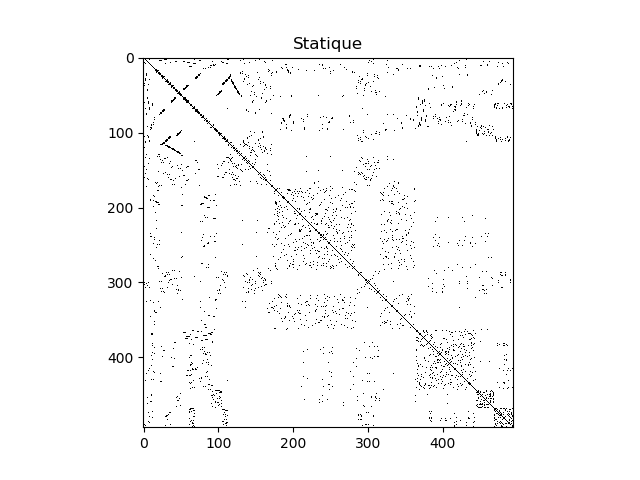
\includegraphics[width = 0.25\textwidth]{matrix/Statique.png}}
\subfloat{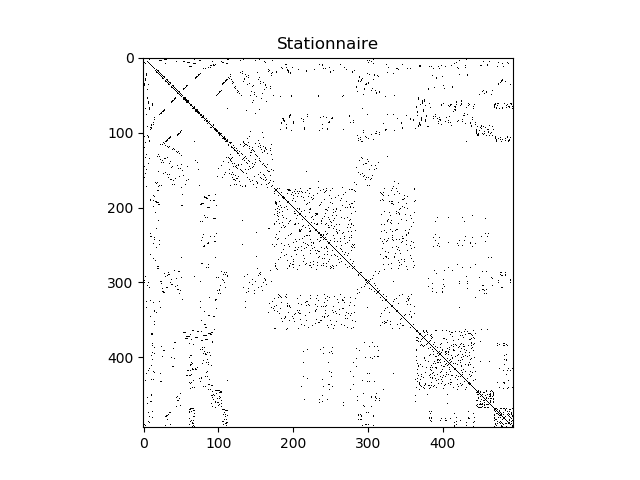
\includegraphics[width = 0.25\textwidth]{matrix/Stationnaire.png}}
\subfloat{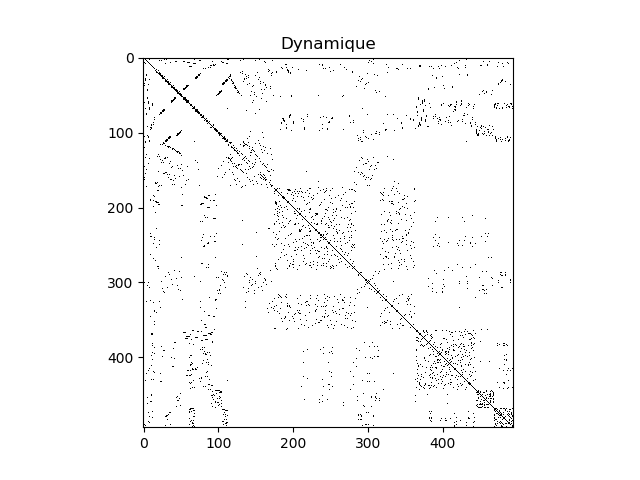
\includegraphics[width = 0.25\textwidth]{matrix/Dynamique.png}}
\subfloat{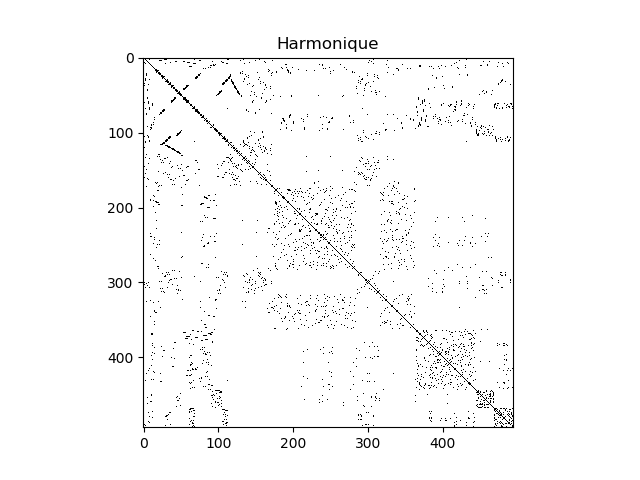
\includegraphics[width = 0.25\textwidth]{matrix/Harmonique.png}}
\end{figure}

\textbf{Hemitienne :}
Seul le régime stationnaire correspond à une matrice Hermitienne. Une matrice Hermitienne est égale à la transposée de sa matrice conjuguée.

\section{Paramètres influençant le conditionnement de \textit{A}}
\subsection{Largeur de l'entrefer}
La largeur de l'entrefer a été choisie entre 0.1 mm et 0.5 cm pour bénéficier de l'effet de l'entrefer sur le flux, ainsi en étant très proche au départ et plus éloigné par la suite, on peut bien remarquer l'effet qu'a l'entrefer sur le champ magnétique lorsque qu'il parcourt le cycle.
\begin{center}
    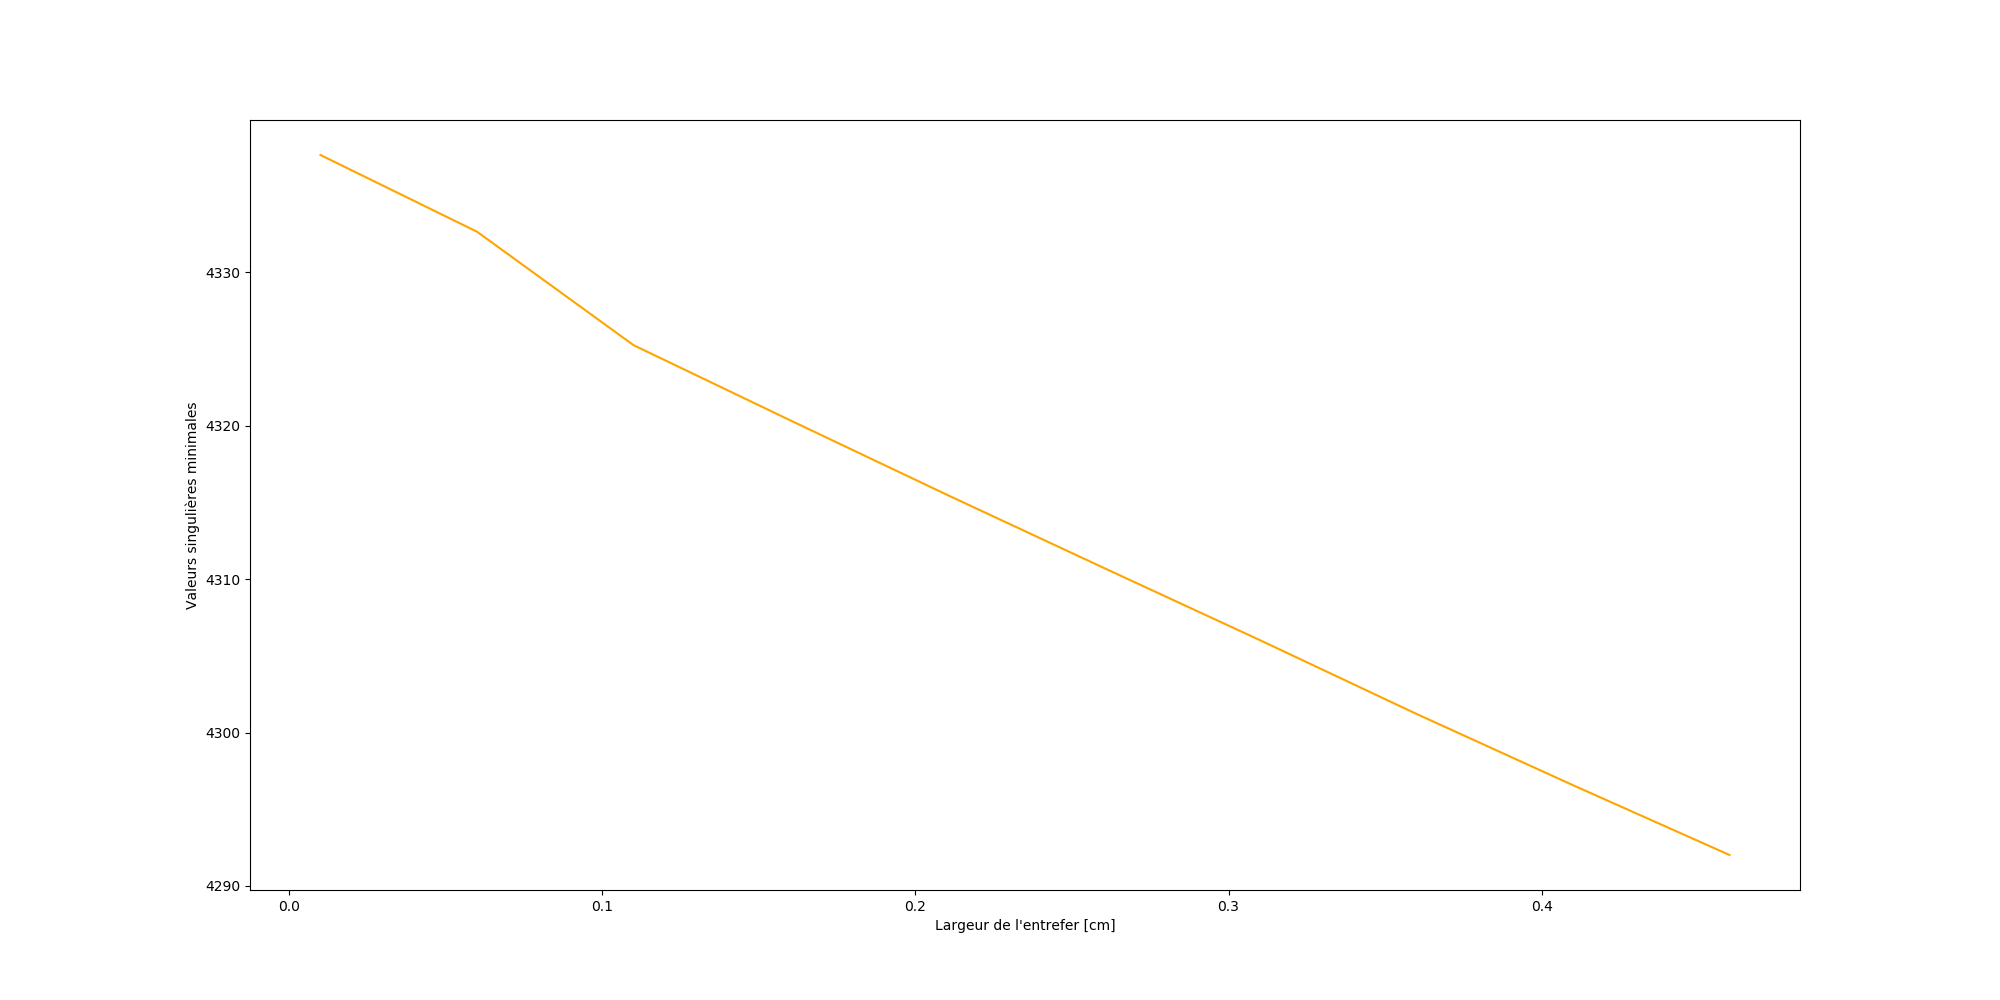
\includegraphics[width = 10cm]{influences/plots/gap_min.png}
    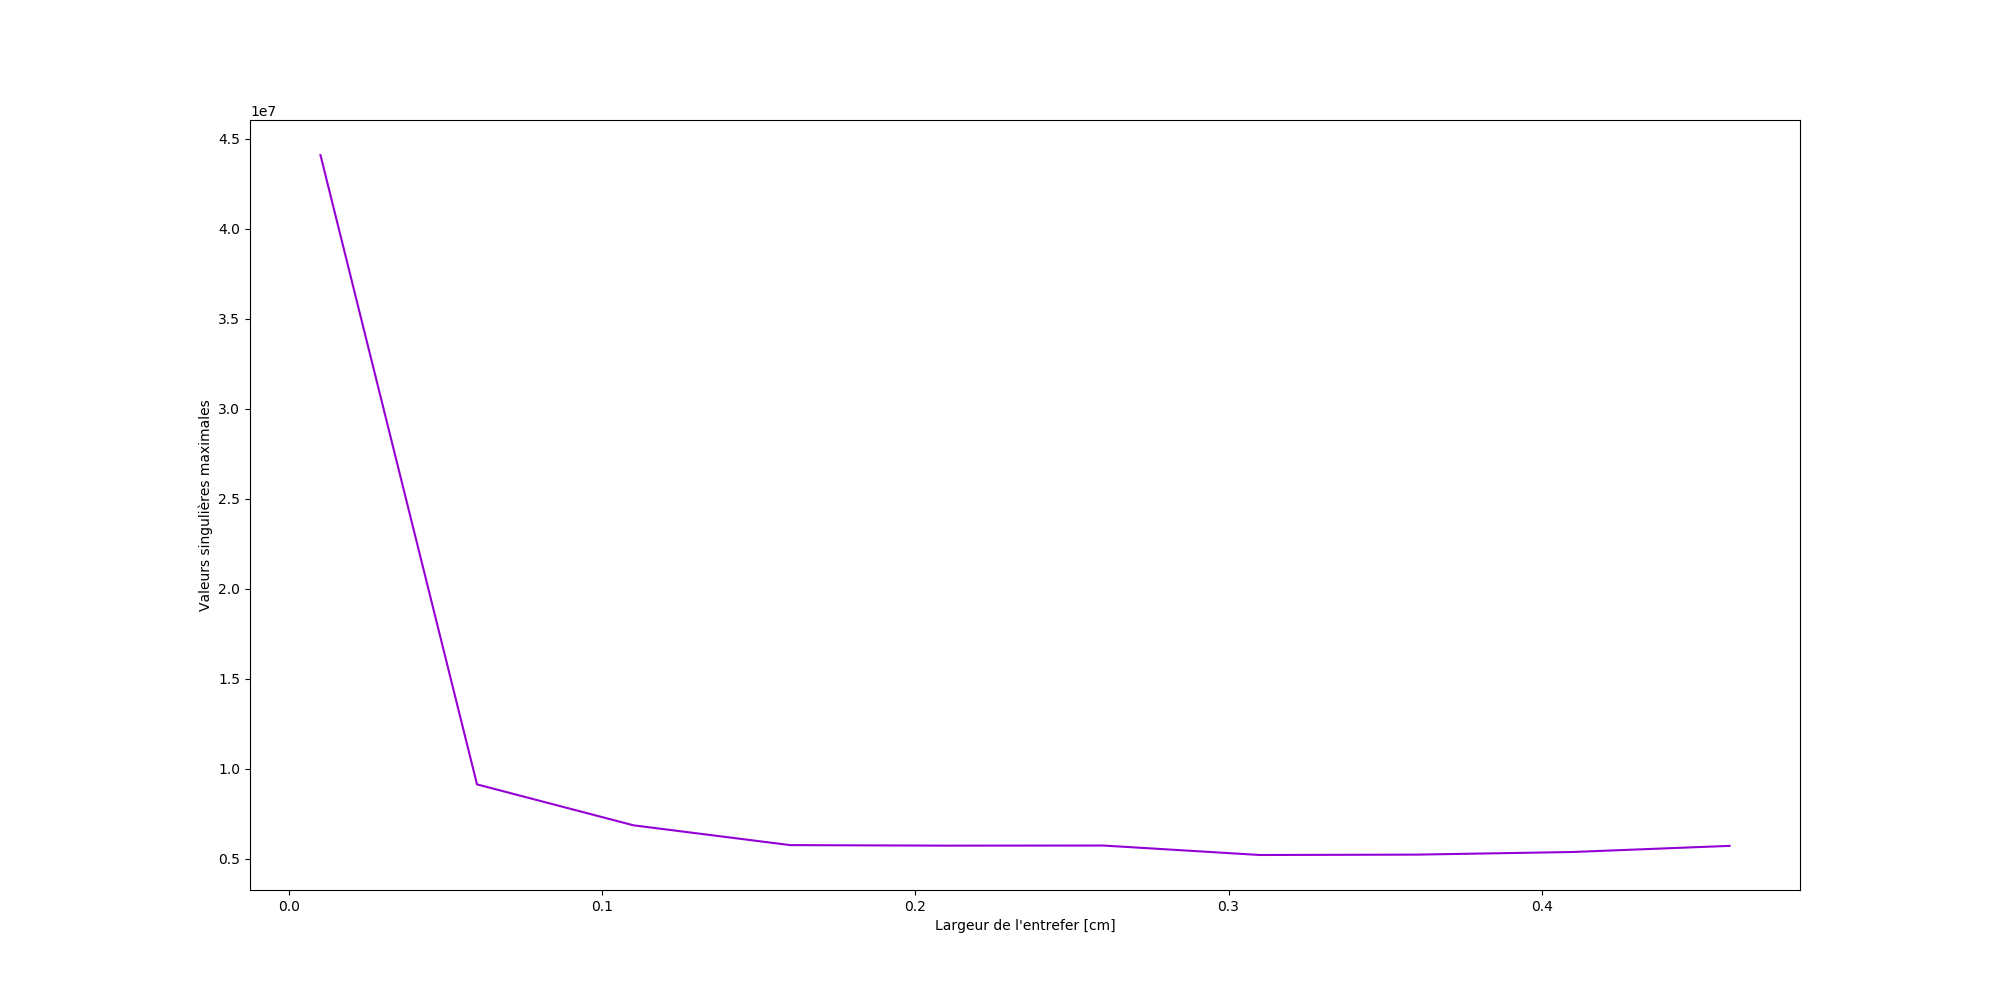
\includegraphics[width = 10cm]{influences/plots/gap_max.png}
    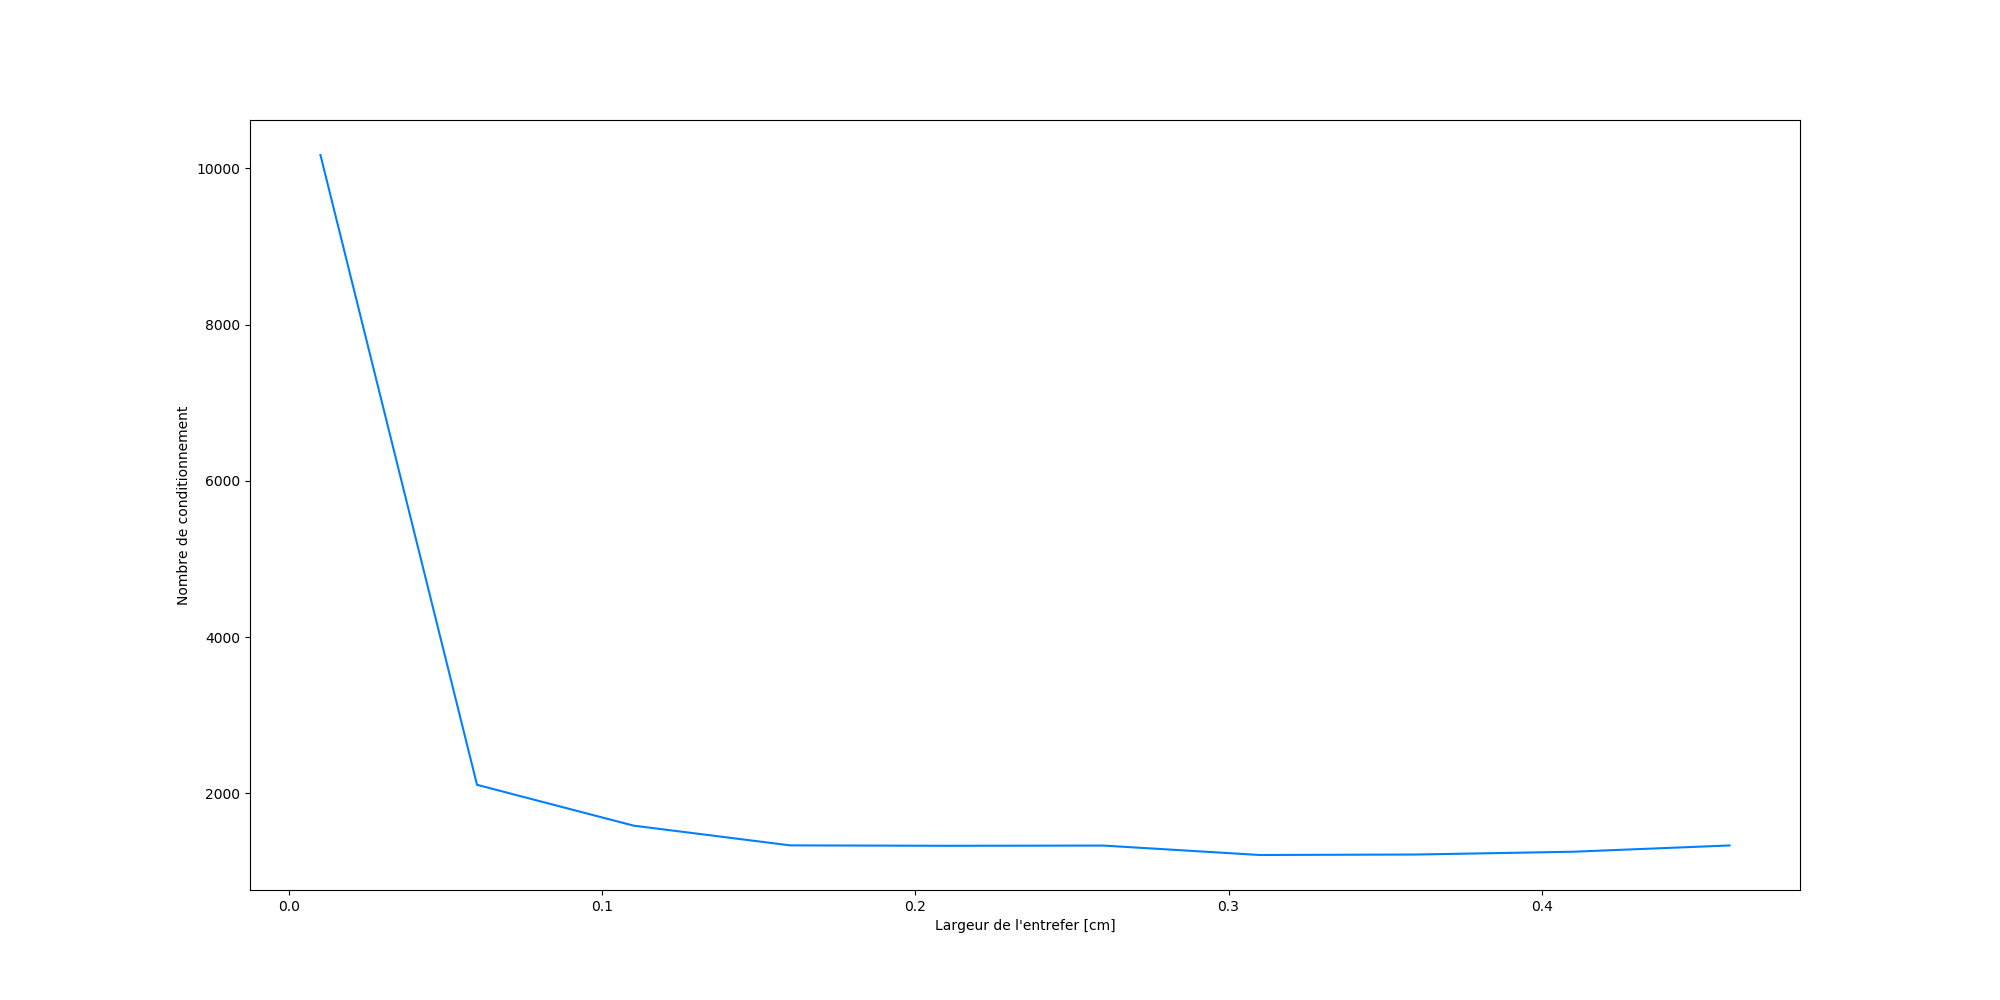
\includegraphics[width = 10cm]{influences/plots/gap_k.png}
\end{center}

\subsection{Perméabilité relative}
Les perméabilités relatives ont été choisies pour parcourir un panel naturel allant de l'air au cobalt \{1, 250\}. Ainsi, on peut voir l'effet de $\mu_r$ sans partir dans des valeurs extrêmes qui ne donnerait pas un bon ressenti de l'effet de ce dernier sur les valeurs singulières.
\begin{center}
    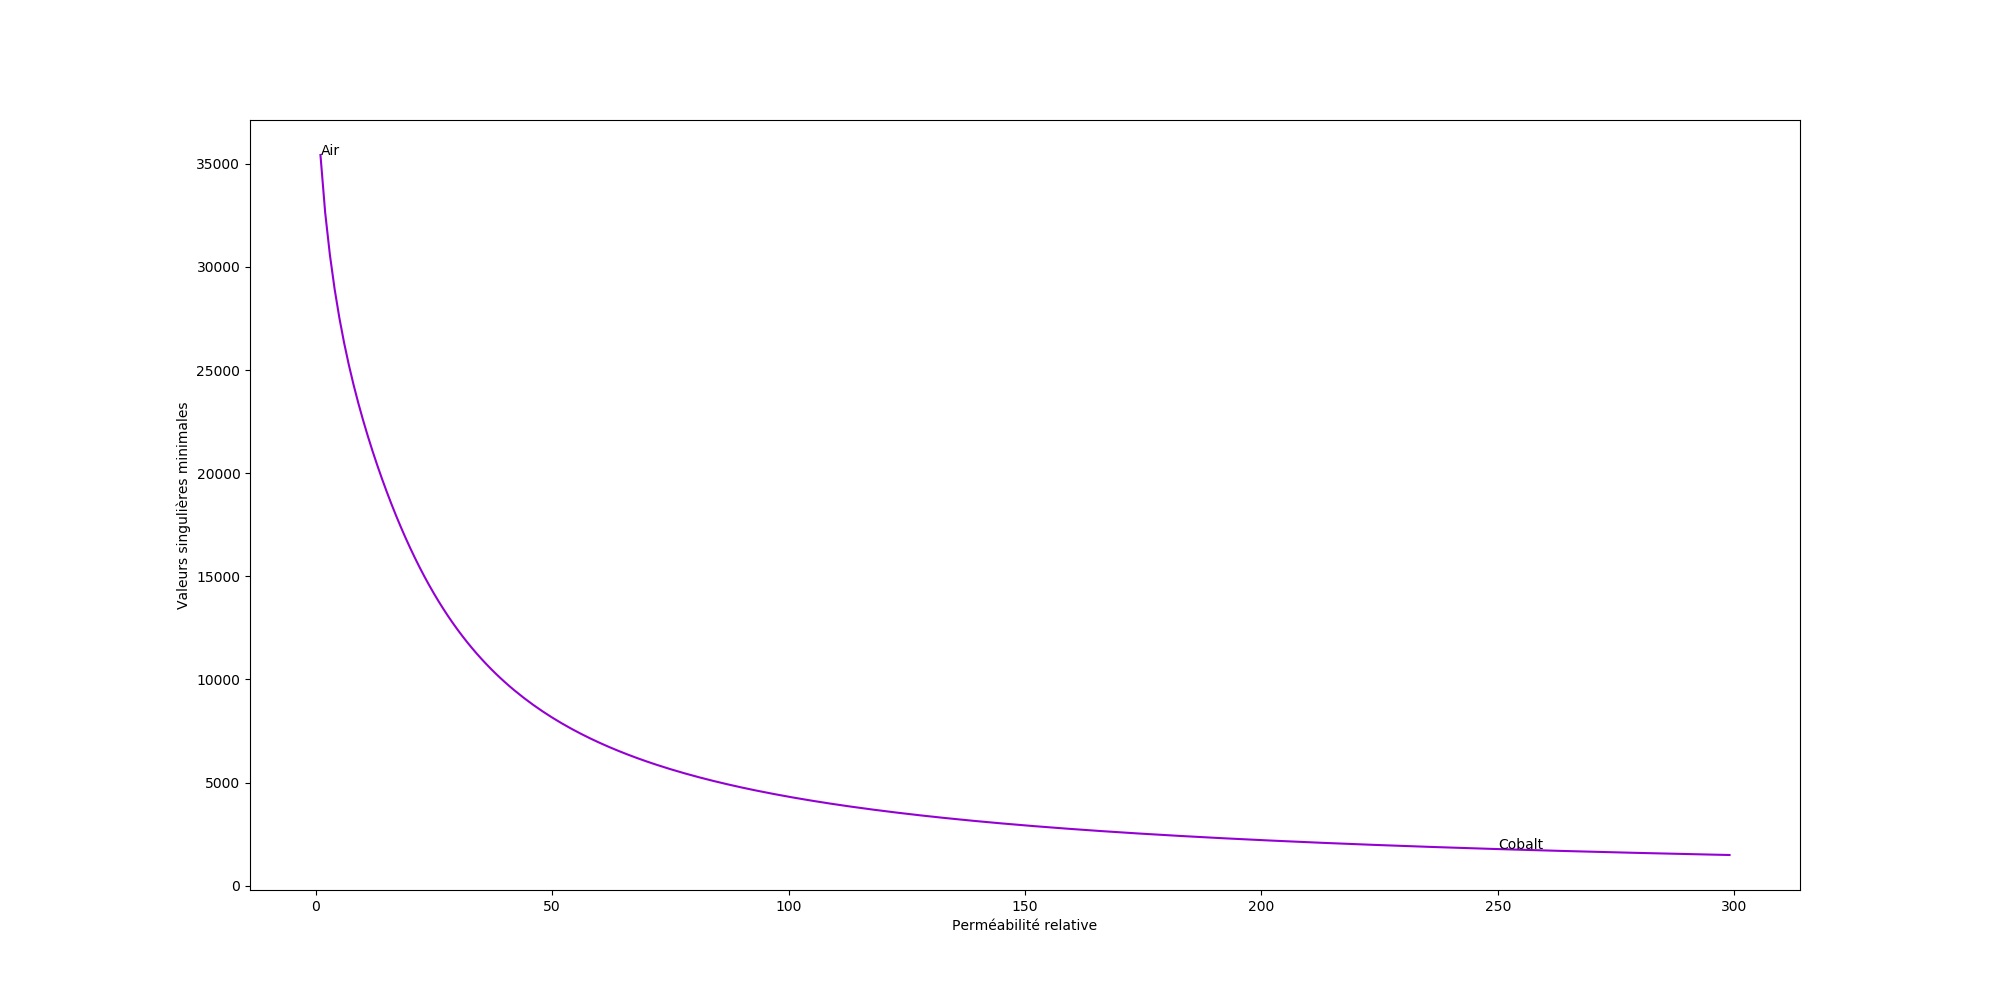
\includegraphics[width = 10cm]{influences/plots/perm_min.png}
    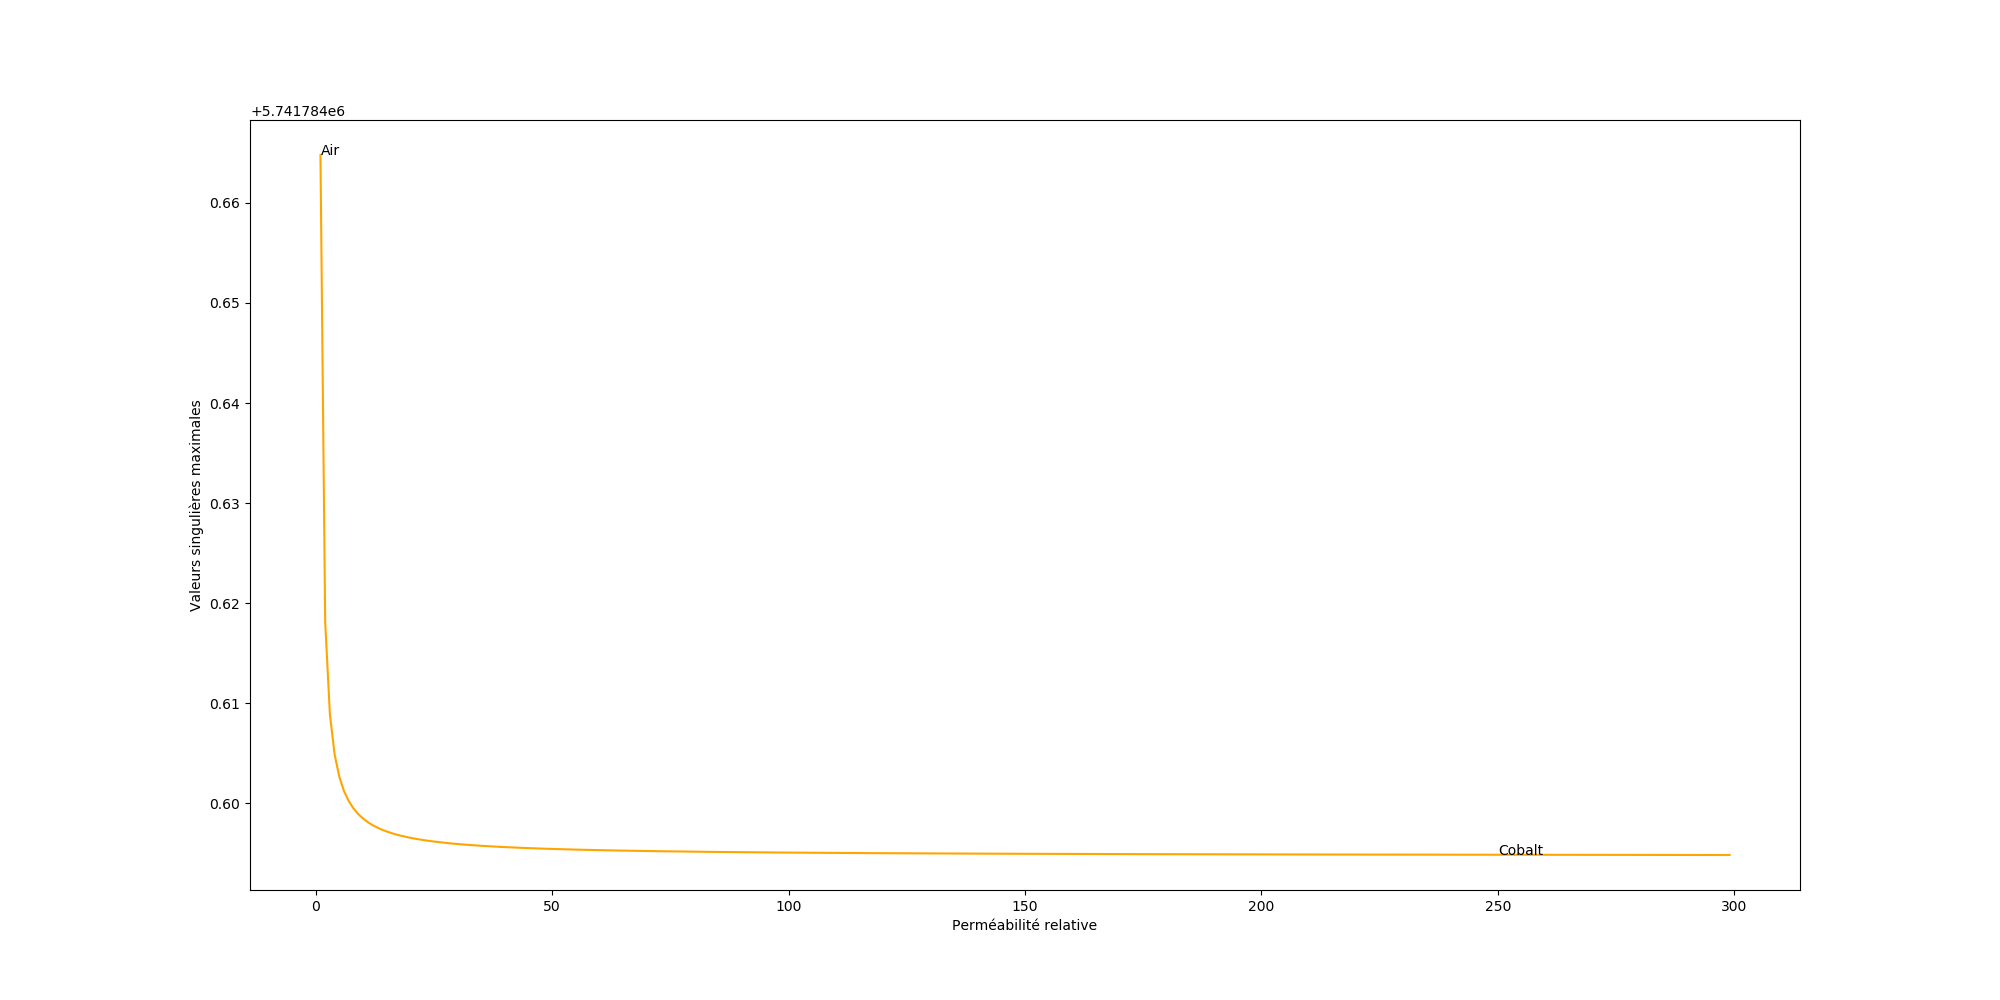
\includegraphics[width = 10cm]{influences/plots/perm_max.png}
    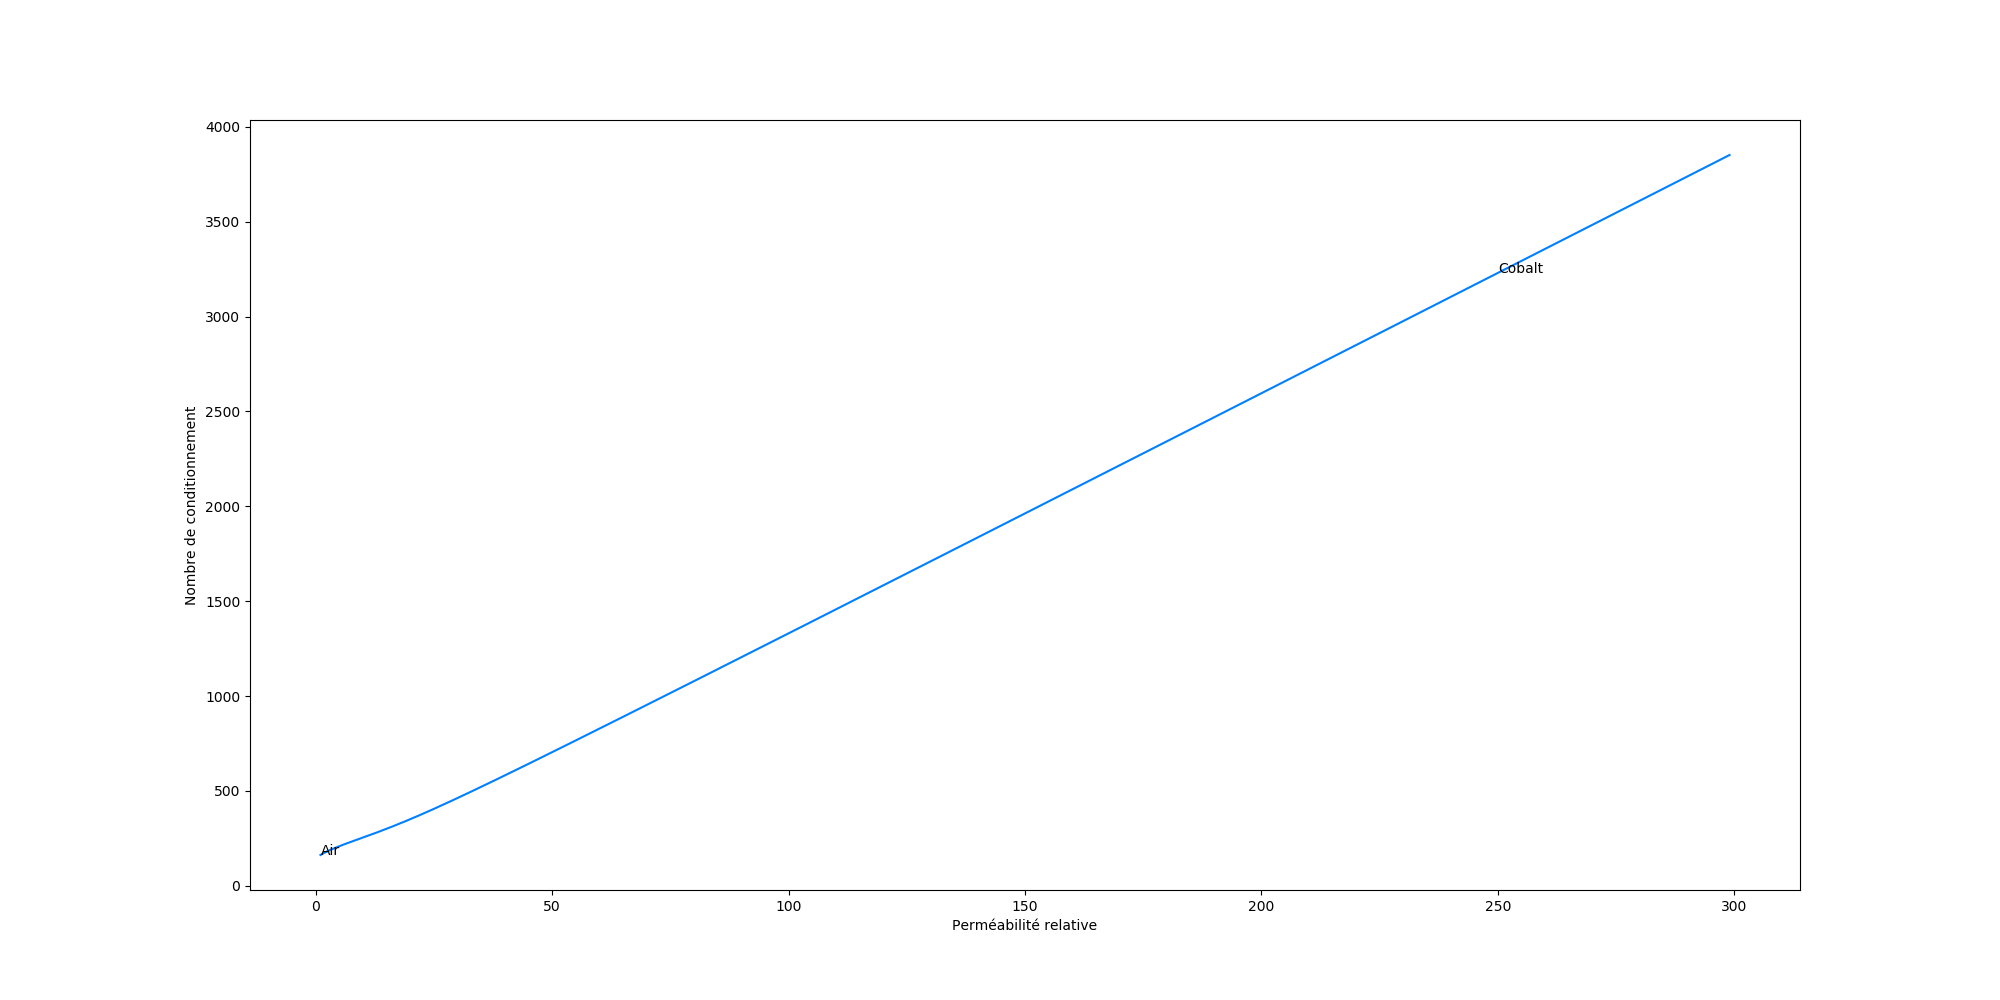
\includegraphics[width = 10cm]{influences/plots/perm_k.png}
\end{center}

\subsection{Maillage}
L'entièreté de la possibilité du maillage a été testée, ainsi \python{ref} prend les valeurs allant de 1 à 5 et les noeuds allant de 393 à 5524.
\begin{center}
    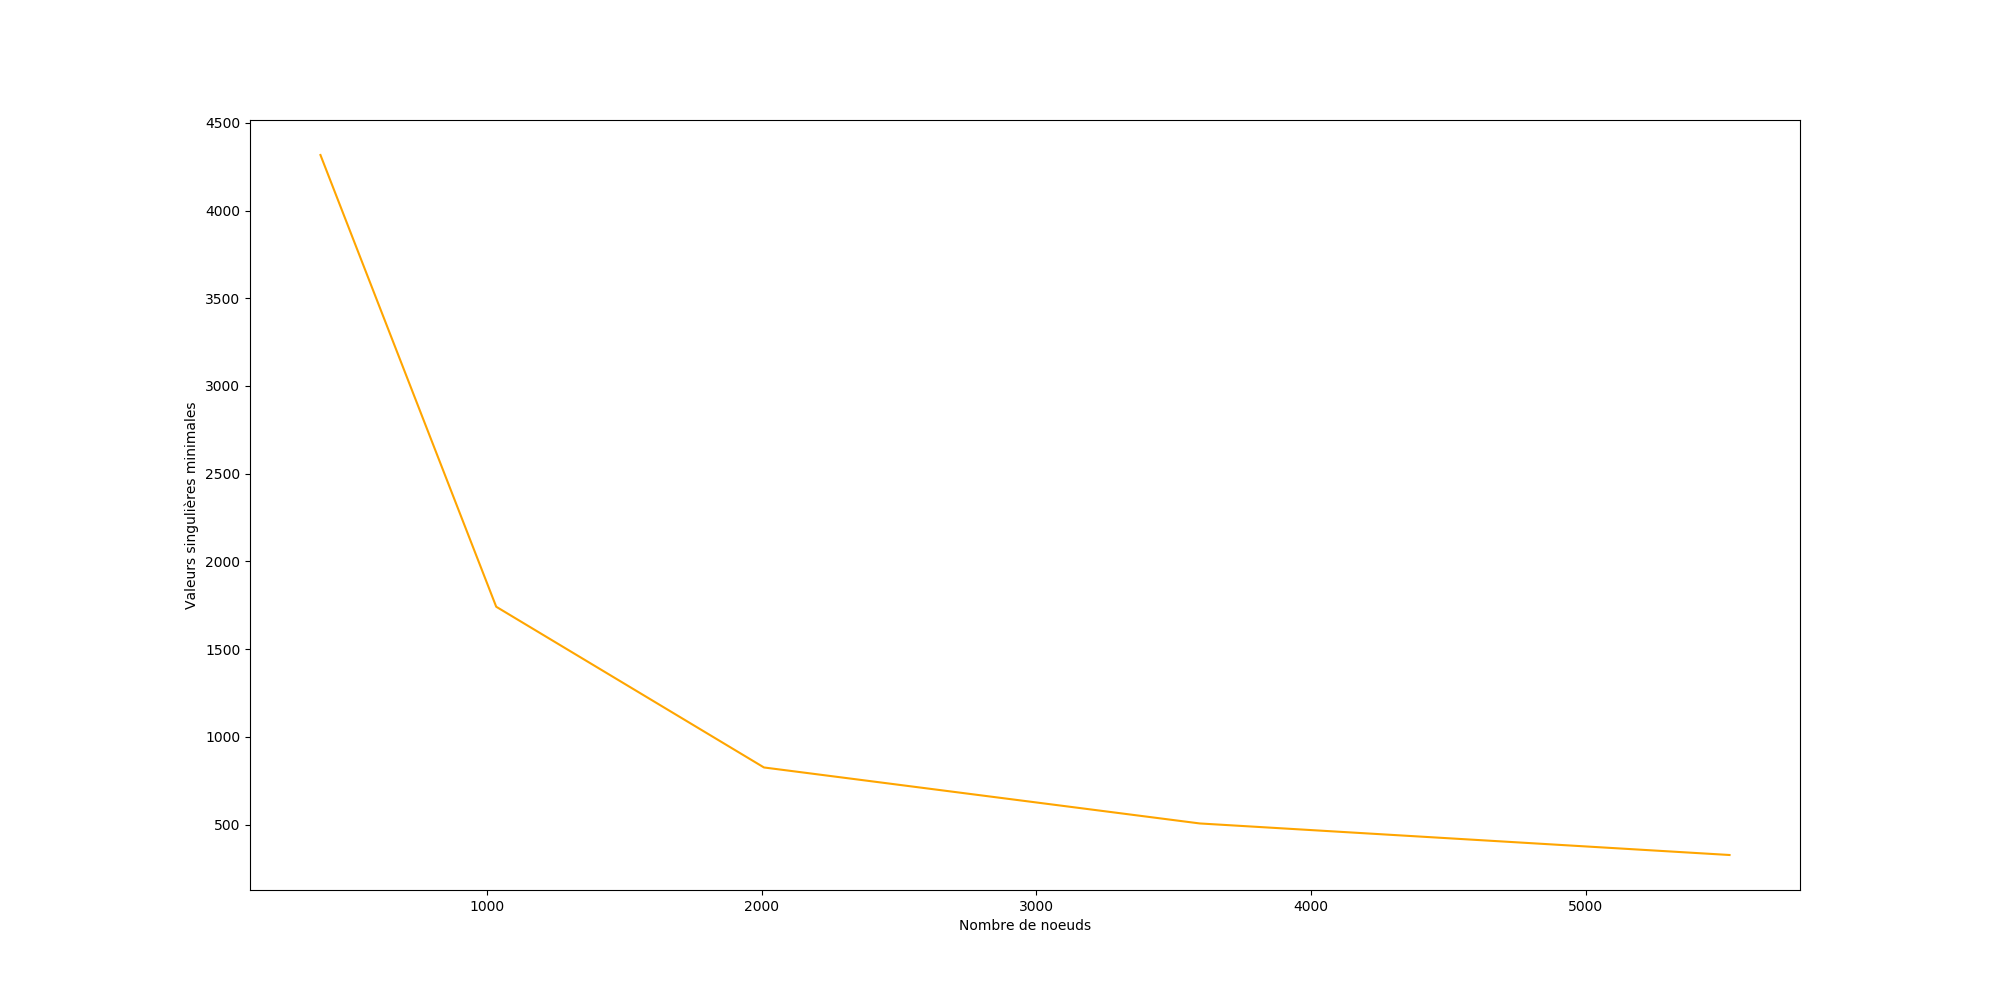
\includegraphics[width = 10cm]{influences/plots/ref_min.png}
    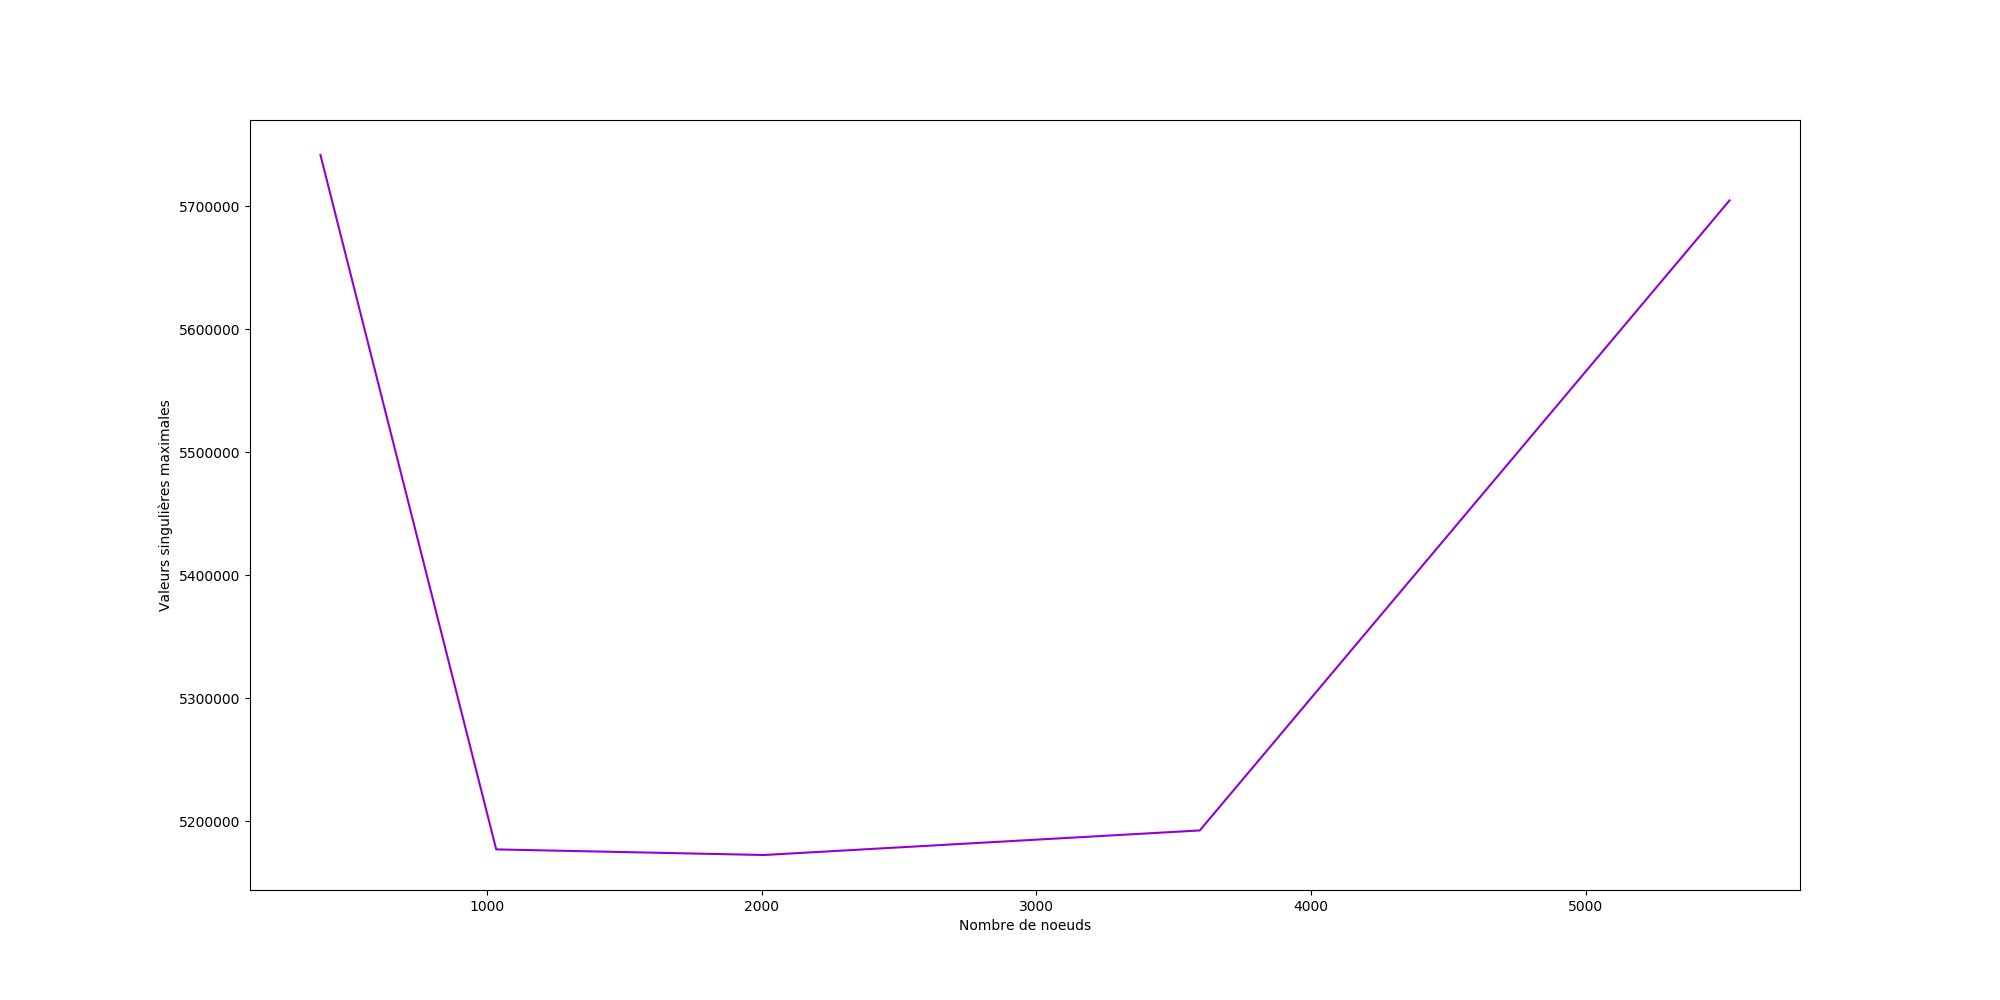
\includegraphics[width = 10cm]{influences/plots/ref_max.png}
    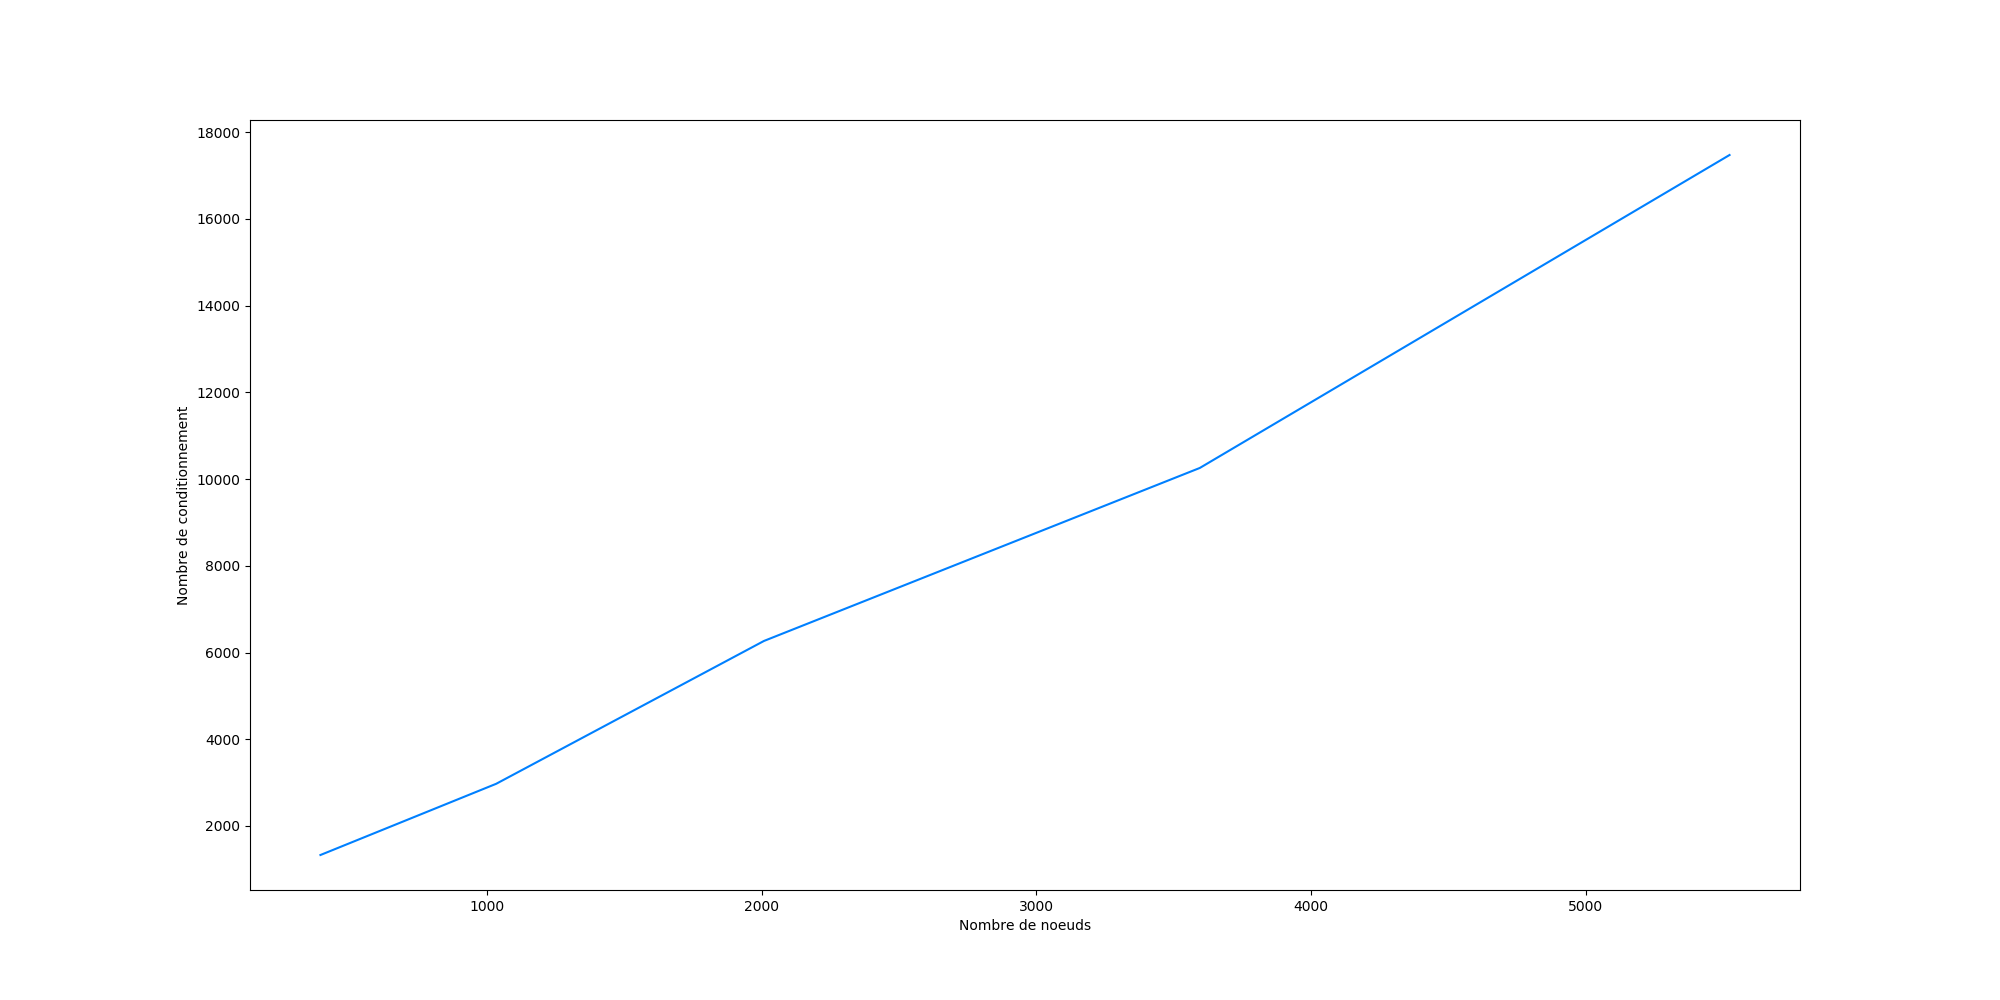
\includegraphics[width = 10cm]{influences/plots/ref_k.png}
\end{center}

\section{Interprétation}

Par analogie avec la poutre encastrée, le courant joue ici le rôle de la force nodale et le flux joue le rôle de la déformée de la poutre. Ainsi, pour chercher les valeurs singulières minimales et maximales, il faut appliquer un courant en chaque noeud indépendemment et visualiser sur quel noeud ce courant produit le plus et le moins de flux. L'action maximale sera obtenue lorsque l'on appliquera un courant au milieu de la bobine centrale (contenue dans l'entrefer) et l'action minimale sera obtenue lorsque l'on applique un courant dans la bobine située en dehors de l'entrefer. En effet, l'entrefer va avoir pour objectif de faire circuler les lignes de champ magnétique qui vont ainsi avoir une plus grande amplitude.
\subsection{Largeur de l'entrefer}

Comme nous pouvons le remarquer sur le graphe ci-dessus, le nombre de conditionnnement diminue à force que le 'gap' de l'entrefer augmente. Comme submentionné, l'entrefer va avoir un effet amplificateur sur les lignes de champs qui vont parcourir un cycle. Lorsque le 'gap' est très petit, les lignes de champs sont favorisées à parcourir ce cycle, ce qui n'est pas le cas lorsque l'entrefer s'éloigne. Le flux étant plus grand lorsque le 'gap' est petit, une même perturbation des données ammène à une plus grande erreur de la solution.
\subsection{Perméabilité relative}

Selon les équations $\overrightarrow{B} = \mu\overrightarrow{H}$ et $\mu = \mu_0\mu_r$, nous pouvons remarquer que le champ magnétique $\overrightarrow{B}$ augmente lorsque la perméabilité augmente. Ainsi, comme au point précédent, lorsque la perméabilité relative augmente, le champ magnétique augmente et donc le conditionnement augmente également.
\subsection{Maillage}

Lorsque nous utilisons un maillage peu raffiné, les éléments sont plus grands, le calcul par élément est donc moins précis et résulte d'une 'moyenne'. Plus le raffinement est élevé et plus 'la moyenne' pour l'élément contenant le flux maximal sera grande. Ainsi, le conditionnement augmente avec le raffinage dû à la précision et les extrêmités des valeurs de flux.
\end{document}
